\chapter{Evaluation}
\section{Ergebnis}
\subsection*{Max Lenk, Christoph Meise}
Insgesamt kam es im Verlauf der Arbeit zu einer Vielzahl von unerwarteten Schwierigkeiten und Verzögerungen. Die Anfangsphase war hauptsächlich von technischen Hardwareproblemen geprägt. Dabei war zuerst die Drohne und anschließend die Grafikkarte des Laptops defekt. \newline
Auch softwareseitig kam es zu Verzögerungen. Die externen Projekte SVO und REMODE setzen eine sehr spezielle Umgebungskonfiguration voraus. So musste durch einen iterativen Prozess die richtige Kombination aus Betriebssystemversion, ROS Distribution und Grafikkartentreiber herausgefunden werden. Hinzu kommen eine Vielzahl von nötigen Abhängigkeiten, wie beispielsweise NVIDIA CUDA, deren Versionen wiederum untereinander kompatibel sein mussten.  \newline
Auch die Kalibrierung der Kamera und die Konfiguration der Parameter stellte eine Herausforderung dar. Der Grund dafür sind Abweichungen in der Projektumgebung. SVO und REMODE sind dafür entwickelt worden, um die Bilder einer hochauflösenden Weitbildkamera auszuwerten, welche nach unten gerichtet ist. In dieser Arbeit wurde jedoch nur eine 720p Kamera mit 92 Grad Blickfeld verwendet, welche nach vorn gerichtet ist. Weiterhin muss die Kamera gelten unterschiedliche Bedingungen mit der simulierten und der realen Drohne. \newline
Letztendlich konnte eine passende Konfiguration der Parameter für die Simulation gefunden werden, bei der richtigen Drohne war jedoch jeglicher Versuch zur Gewinnung von Tiefenbildern gescheitert. \newline
Die Ausarbeitungen zu dem Assistenzsystem haben zu dem Ergebnis geführt, dass im Rahmen dieser Arbeit eine Implementierung unter den gegebenen Anforderungen nicht möglich ist. Hauptsächlich schuld ist dafür die mangelnde Performance von SVO und REMODE in der Projektumgebung, wodurch Tiefeninformationen nur langsam, ungenau und instabil gewonnen werden können. Da die Entwicklung eines Assistenzsystems auf Objekterkennung basiert, müssen aus den verschwommenen Tiefenbildern möglichst genau Objekte wie z.B. Türen erkannt werden. Die im Rahmen dieser Arbeit betrachteten Herangehensweisen für diese Problematik haben sich alle als nicht valide herausgestellt. Im Speziellen gibt es keine verwendbaren Algorithmen in der Point Cloud Library, wodurch eine Realisierung mit enorm hohem Eigenaufwand verbunden wäre. Auf Grund der vielen Verzögerungen und dem begrenzten zeitlichen Rahmen der Arbeit, war dies nicht mehr möglich.
Die Anforderung, die Gestensteuerung der Drohne von C\# unter Windows auf C++ unter Ubuntu zu migrieren konnte jedoch erfolgreich umgesetzt werden.

\section{Ausblick}
\subsection{Andere Simulatoren}
Die Simulationsumgebung Gazebo ist nicht die einzig verfügbare Umgebung zur Simulation von Quadrocoptern. Jedoch bringt sie durch die einfache Anbindung von ROS einige Vorteile mit sich. Damit gehen allerdings auch Nachteile einher. So sind die Kameraeingaben nicht sehr realistisch und Szenarien die in der Simulation funktionieren müssen in der Realität nicht funktionieren. Ebenso ist das Flugverhalten in manchen Situation nicht realitätsgetreu und kann zu verfälschten Ergebnisse führen. Um diesem Vorzubeugen ist es ratsam die Resultate mit anderen Simulationen vergleichen. Eine aktuelle Simulationsumgebung zur Simulation von Quadrocoptern ist der AirSim von Microsoft.\cite{airsim} Ursprünglich entwickelt um Trainingsdaten zum maschinellem Lernen sammeln, kann er ebenfalls auch für herkömmliche Simulation verwendet werden. Aktuell ist allerdings nur für Windows Betriebssysteme verfügbar. \cite{airsimpaper} Er bietet eine fotorealistische Umgebung und ein akkurates Flugverhalten, dadurch ist der Simulator besonders für Demos und Showcases besser geeignet. \newline
Es existieren weiterhin andere Simulatoren, allerdings sind die meisten spielerisch veranlagt und bieten keine programmatische Schnittstelle, weshalb sie für den Zweck des Anwendungsfalles nicht sinnvoll verwendet werden können.
\begin{figure}[ht]
	\centering
	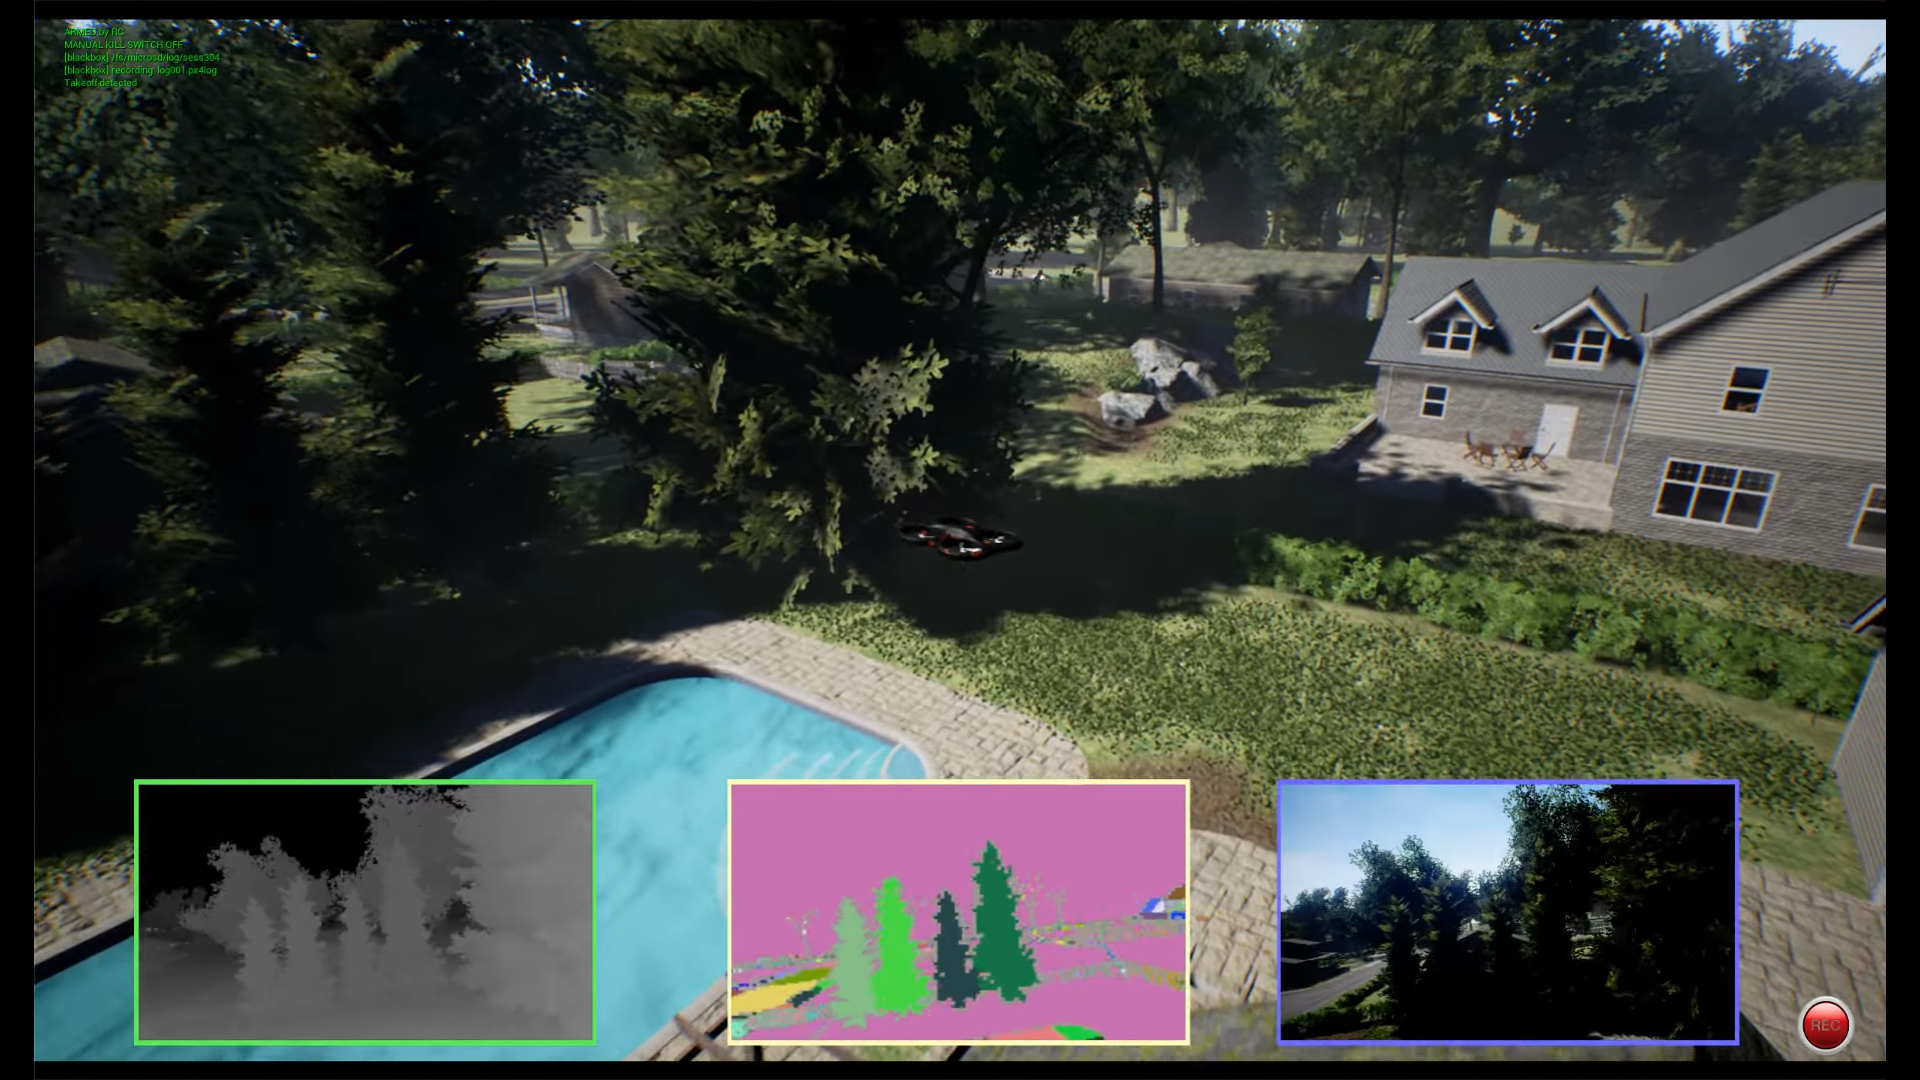
\includegraphics[scale=0.28]{Bilder/airsim.png}
	\label{fig:airsim}
	\caption{AirSim von Mircosoft in Aktion\cite{airsim}}
\end{figure}
%beide



\subsection{Assistenzsystem}
Wie bereits beschrieben, konnte im Rahmen dieser Arbeit keine Lösung für ein Assistenzsystem gefunden werden. Die Bearbeitung hat jedoch diverse Erkenntnisse hervorgebracht, welche für weitere Arbeiten relevant sein können. \newline
Eines der Hauptprobleme besteht in der Verwendung von den externen Projekten SVO und REMODE. Diese sind für eine bessere Kamera ausgerichtet, welche vor allem nach unten gerichtet ist. Es hat sich herausgestellt, dass die Software nicht funktioniert, sobald die Drohne sich um die eigene Achse dreht, oder nach vorne bzw. hinten fliegt. Um dieses Problem zu beheben, könnte entweder der Code angepasst werden, oder eine eigene Implementierung vorgenommen werden. \newline
Weiterhin könnte es sinnvoll sein sich genauer mit den Algorithmen der Point Cloud Library zu beschäftigen. Hierbei ist hauptsächlich die Objekterkennung in den Tiefenbildern problematisch. \newline
Insgesamt ist jedoch die Grundvoraussetzung für ein funktionierendes Assistenzsystem, dass die darauf basierenden Tiefeninformationen sowohl aktuell, als auch möglichst exakt sind. Anderenfalls ist das damit verbundene Fehlerpotential zu hoch, wodurch die Steuerung der Drohne negativ beeinflusst wird.